\documentclass{beamer}
\usepackage[italian]{babel}
\usepackage[utf8]{inputenc}
\usepackage[T1]{fontenc}
\title{Complementi alle lezioni di Fisica per la classe 1C}
\author{Giorgio Barone}
\date{Milano, 10/02/2023}
\institute[]{Liceo Scientifico "Alessandro Volta"}
\logo{
\includegraphics[width=15mm]{logoLiceoVolta.png}}
\usetheme{Berkeley}

\usecolortheme{default}
\setbeamercovered{dynamic}
\theoremstyle{definition}
\newtheorem{definizione}{Definizione}
\theoremstyle{plain}
\newtheorem{teorema}{Teorema}

\begin{document}
\begin{frame}
\maketitle
\end{frame}
\begin{frame}
\frametitle{La misura di una grandezza fisica}
\tableofcontents
\end{frame}

\section{La Misura}

\begin{frame}
\frametitle{La misura di una grandezza}
Sia $X$ una grandezza fisica (spazio, velocità, densità,...)

chiamiamo \emph{Misura della grandezza $X$} la scrittura : 
\begin{equation}
X = (X_M \pm \Delta X),
\label{1}
\end{equation}
dove $X_M$ è il \emph{Valor Medio} e $\Delta X$ è l'\emph{errore assoluto} o \emph{Incertezza assoluta}.

Per esempio su una scala graduata in una generica unità di misura $s$ leggiamo il valore $14.5$ come valore più vicino a quello reale, ma non siamo sicuri se in realtà il \emph{valore vero} della grandezza sia compreso tra due valori estremi $X_{max} = 14.7 s$ e $X_{min} = 14.3 s$.
\begin{figure}
  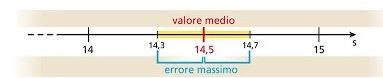
\includegraphics[width=0.8\columnwidth]{errore_assoluto1.jpg}
\end{figure}

\end{frame}

\begin{frame}
\frametitle{semidispersione come errore assoluto}
Allora la scrittura (\ref{1}) equivale a dire che il valore vero è compreso tra $X_{max}$ e $X_{min}$, nel senso che $\Delta X$ è proprio la \emph{semidispersione} $(X_{max} - X_{min})/2$ 
\begin{equation}
\Delta X = \frac{X_{max} - X_{min}}{2},
\label{2}
\end{equation}
ed allo stesso modo il valore medio:
\begin{equation}
X_M = \frac{X_{max} + X_{min}}{2},
\label{3}
\end{equation}
che nell'esempio precedente diventa rispettivamente:
$\Delta X = 0.2 s$ e $X_M = 14.5s$.

In generale, ogni volta che siamo incerti nell'associare un errore assoluto nelle misure che facciamo (per esempio nelle misure ripetute di una grandezza) per non rischiare di sbagliare (anche se potremmo sovrastimare l'errore) associamo in generale la semidispersione all'Incertezza assoluta.

\end{frame}

\section{Propagazione dell'errore}

\begin{frame}
\frametitle{La propagazione dell'errore nella somma}
Nel caso in cui avessimo due misure tra loro \emph{dimensionalmente omogenee}, cioè entrambe aventi esattamente la stessa dimensione fisica (entrambe lunghezze ed espresse nella stessa unità di misura, non per forza metri, per fare un esempio...) ci si pone il problema di associare l'errore assoluto appropriato alla \emph{misura indiretta} della loro somma o prodotto.

Per esempio se abbiamo un metro troppo piccolo per misurare la lunghezza di un grande tavolo, ma comunque prendiamo accuratamente due misure dirette:
$x = (100.0 \pm 0.1) cm$ e $y = (34.3 \pm 0.1) cm$ è banale calcolare che il valor medio della somma, cioè
$(x + y)_M = 100.0cm + 34.3cm = 134.3 cm$, ma in generale non sappiamo che errore dobbiamo associare alla grandezza $(x+y)$...
\end{frame}

\begin{frame}
\frametitle{L'incertezza assoluta nella somma}
Come detto prima, visto che non siamo sicuri su che errore associare alla grandezza somma (intesa come somma algebrica, cioè addizione e sottrazione), calcoliamo la semidispersione della somma di $x + y$:
\begin{equation}
\Delta (x+y) = \frac{ (x+y)_{max} - (x+y)_{min} }{2}
\label{4}
\end{equation}
$\
(x+y)_{max} = x_{max} + y_{max} = x + \Delta x + y + \Delta y
\ $

$\
(x+y)_{min} = x_{min} + y_{min} = x - \Delta x + y - \Delta y
\ $

ed in questo modo, sfruttando la (\ref{4}), otteniamo

\begin{equation}
\Delta (x+y) = \frac{2 \Delta x + 2 \Delta y}{2} 
             = \Delta x + \Delta y 
\label{5} 
\end{equation}
\begin{theorem}
L' incertezza assoluta della somma algebrica di due misure è la somma delle incertezze assolute
\end{theorem}
\end{frame}


\begin{frame}
\frametitle{L'errore nel prodotto di due misure}
Supponiamo ora di voler calcolare una misura indiretta di una grandezza la cui espressione si ottiene tramite il prodotto algebrico (moltiplicazione o divisione) di due misure dirette. Per esempio il calcolo dell' \emph{area} di un tavolo date le misure delle lunghezze dei lati o la densità di una quantità di liquido (massa diviso il volume).

\begin{figure}
  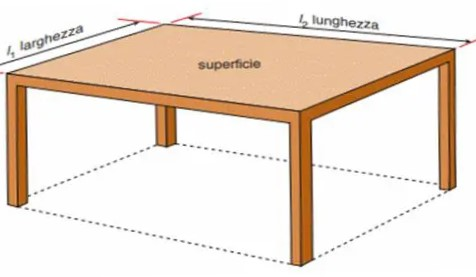
\includegraphics[width=0.8\columnwidth]{Tavola.jpg}
\end{figure}


\end{frame}

\begin{frame}
\frametitle{somma di errori relativi}
L'\emph{errore relativo} è definito come 
\begin{equation}
\varepsilon _{r} (X) = \frac{\Delta X}{X}
\label{6}
\end{equation} 
E la grandezza la cui misura \emph{indiretta} è il prodotto sia $z = xy$.

Per calcolare il valore medio del prodotto di due grandezze, risulta banale considerare il prodotto dei valori medi:
\begin{equation}
z_{M} = x_M y_M,
\label{7}
\end{equation}
ma per quanto riguarda l'incertezza assoluta, come abbiamo fatto in precedenza ed in generale essa è data dalla $\bold{semidispersione}$


\end{frame}
\end{document}